%------------------------------------------------------------------------------

\chapter{Θεωρία}
\label{chapter3} 

Το κεφάλαιο αυτό θα αναλύσει ότι χρειάζεται να ξέρει ο αναγνώστης για να
κατανοήσει το κεφάλαιο της υλοποίησης. Αρχικά θα περιγράψουμε εκτενέστερα την
διαδικασία που ακολουθείται στο σύστημα RPython για την μεταγλώττιση (π.χ. του
PyPy), έτσι ώστε να ξέρει ο αναγνώστης σε ποιο "χρονικό" σημείο θα λάβει χώρα το
εγχείρημά μας. Έπειτα θα παραθέσουμε με λεπτομέρεια την θεωρία της μεθόδου που
θα υλοποιήσουμε.

%------------------------------------------------------------------------------

\section{Διαδικασία Μεταγλώττισης στο σύστημα RPython}

\subsection{Επισκόπηση}

Ο σκοπός του συστήματος και του \textit{toolchain} του RPython είναι να
μεταφράσει προγράμματα (κυρίως μεταφραστές) γραμμένα σε RPython με
αποτελεσματικότητα ανεξάρτητα με το ποια πλατφόρμα είναι το target του. Το
default target είναι το \textit{C backend} (παραγωγός κώδικα C) και σε αυτό θα
αναφερόμαστε όταν δίνουμε παραδείγματα.

Το σύστημα στην πραγματικότητα δεν βλέπει ποτέ κανονικό κώδικα Python ή δέντρα,
αλλά ξεκινά με \textit{αντικείμενα κώδικα} (code objects) βασισμένα στις
συναρτήσεις που έχουν δοθεί ως είσοδος και τα μετατρέπει με \textit{abstract
interpretation}\cite{CousotCousot77}\cite{debray1995abstract} σε γραφήματα ροής.
Η βασική δηλαδή δομή δεδομένων (unit) πάνω στην οποία δουλεύει το σύστημα
επομένως είναι τα γραφήματα ροής (σε ΠΩΣ ΔΙΑΛΟ ΛΕΓΕΤΑΙ) βασισμένα σε function
code objects. Ένα γράφημα για κάθε συνάρτηση. Αυτά τα γραφήματα είναι απλώς ένας
ακόμα τρόπος αναπαράστασης του προγράματος, αλλά πιο κατάλληλος για
"αφαιρετικές" εργασίες μεταγλώττισης και βελτιστοποίσης (π.χ. εξαγωγή
τύπων\footnote{βλ. type inference}).

Η διαδικασία είναι οργανωμένη σε στάδια (βλ. \ref{figure-1}).

\begin{enumerate}

\item Import \& Flow Analysis. Εδώ ο αρχικός κώδικας φορτώνεται στην μνήμη και
υφίσταται τις βασικές διαδικασίες συντακικής ανάλυσης. Μετατρέπεται αρχικά σε
tokens, έπειτα σε μια ενδιάμεση μορφή (Python bytecode) – όπως σε όλους τους
μεταγλωττιστές – και τέλος στα διαγράμματα ροής του PyPy. Από αυτό το στάδιο και
έπειτα φυσικά βρίσκεται μόνο μέσα στην τοπική μνήμη, σε μια αρκετά "στατική"
μορφή για τα δεδομένα του RPython.

\item Annotator subsystem. Εδώ ενεργοποιούνται οι περισσότερο αφαιρετικές
μέθοδοι ερμηνείας του κώδικα. Μια καθολική ανάλυση, που θα ξεκινήσει από το
σημείο εισόδου του κάθε διαγράματος (entry point), θα "εξάγει" γενικές
πληροφορίες για τον κώδικα και θα συμπεράνει τους τύπους που μπορεί η κάθε
μεταβλητή να φιλοξενήσει κατά το runtime βάσει φυσικά των συμφραζομένων. Μετά
από αυτό το βήμα, έχουμε annotated flow graphs.

\item RTyper. Αυτό το σύστημα χρησιμοποιεί τους \textit{υποσημειώμένους}
είδικούς προσωρινούς τύπους που έχει προσθέσει ο annotator για να μετατρέψει τα
statements και τις εντολές στα γραφήματα σε εντολές χαμηλότερου επιπέδου. Είναι
ουσιαστικά μια γέφυρα μεταξύ των γραφημάτων και των παραγωγών κώδικα.

\item Optimizations. Η βελτιστοποίηση στο PyPy γίνεται εδώ. Το project
περιλαμβάνει – και εφαρμόζει –  μια πληθώρα βελτιστοποιήσεων, όπως αυτά που
αναφέραμε στο κεφάλαιο \ref{chapter2}. Επίσης το δικό μας module θα λάβει χώρα
εδώ.

\item Προετοιμασία Γραφημάτων. Εδώ γίνονται οι τελικές ενέργειες πριν την
παραγωγή κώδικα. Τα γραφήματα εδώ λ.χ. υφίσταντο ανάλυση για τον υπολογισμό
ονομάτων μεταβλητών (για λόγους όπως debugging) κ.α. Σημαντικότερες όμως είναι
οι εξής ενέργειες:

\textbf{Exception transformer:} Ο "μετατροπέας εξαιρέσεων" ενεργοποιείται σε
αυτό το σημείο και θα εισάγει τον απαραίτητο κώδικα για τη διαχείριση των
εξαιρέσεων που τυχαίνει να υπάρχουν.

\textbf{Garbage Collection Transformer:} Εδώ παίρνει σειρά το ειδικό εργαλείο
διαχείρισης "σκουπιδιών μνήμης". Αυτό εκτελεί όποιες ενέργειες χρειάζονται για
την σωστή διαχείριση μνήμης. Αφού η Python είναι πλήρως δυναμική γλώσσα και δεν
απαιτεί από τον προγραμματιστή να διαχειρίζεται την μνήμη που χρειάζεται μόνος
του, είναι απαραίτητη η ύπαρξη ενός υποσυστήματος διαχείρισης σκουπιδιών μνήμης.

\item Code Generation. Εδώ τα ήδη μαρκαρισμένα, σημειωμένα, βελτιστοποιημένα
γραφήματα θα μετατραπούν σε κώδικα μηχανής. Εδώ υπάρχουν πολλοί "γεννήτορες"
κώδικα ανάλογα με τις ανάγκες. Ο βασικότερος και ο πιο σημαντικός είναι ο
παραγωγός κώδικα C. Αρχικά, τα γραφήματα θα μετατραπούν σε άλλα αντίστοιχα,
ανάλογα με τον γεννήτορα και έπειτα αυτά θα μετατραπούν σε κώδικα ανάλογα με την
επιλογή (π.χ σε κώδικα C)

\item Τέλος ο κώδικας αυτός θα οδηγηθεί στον μεταφραστή της εκάστοτε επιλογής
(π.χ. \texttt{gcc}) για να παραχθεί το εκτελέσιμο αρχείο.

\end{enumerate}

\begin{figure}[h]
\centering
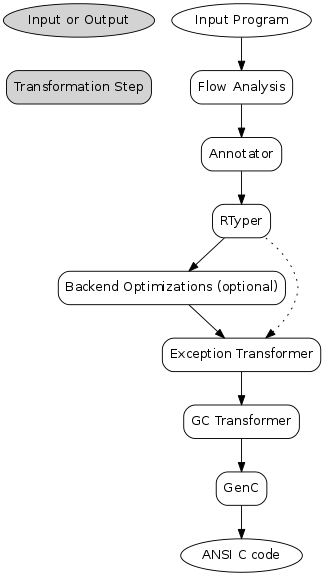
\includegraphics[width=0.5\textwidth]{diagram.png}
\caption{diagram of RPython translation process}
\label{figure-1}
\end{figure}

\subsection{Γραφήματα Ροής}

\subsubsection{Τρόπος δημιουργίας}

Ο σκοπός του κατασκευαστή γραφημάτων (υλοποιημένος στο module
\texttt{rpython.flowspace}) είναι να μετατρέψει τα αντικείμενα συναρτήσεων σε
γραφήματα. Κανονικά οι μεταγλωττιστές παίρνουν μια συνάρτηση και την μετατρέπουν
σε ενδιάμεσο bytecode κώδικα σε κάποια εικονική μηχανή (VM) και έπειτα την
τρέχουν. Στο RPython όμως χρησιμοποιείται ένα \textit{abstract interpretation}
το οποίο λειτουργώντας αφαιρετικά μετατρέπει τον ενδιάμεσο κώδικα στα βασικα
\texttt{ Block}, τα οποία περιέχουν όλες τις εντολές οι οποίες επιδρούν πάνω σε
αντικείμενα Python. Το αποτέλεσμα της κάθε εντολής αποθηκεύεται προσωρινά σε μια
μεταβλητή η οποία μπορεί να χρησιμοποιηθεί στις επόμενες. Για παράδειγμα βλ.
\ref{figure-2} το οποίο είναι ένα γράφημα μιας απλής συνάρτησης με ένα if
branch. Φαίνεται η γενική εικόνα των γραφημάτων, το branch καθώς ο τρόπος που
επαναχρησιμοποιούνται οι προσωρινές μεταβλητές αποτελεσμάτων ανάλογα με τις
ανάγκες.

\begin{figure}[h]
\centering
\includegraphics[width=0.5\textwidth]{simple-func.png}
\caption{simple function flow diagram}
\label{figure-2}
\end{figure}

Ο κατασκευαστής "κλείνει" ένα \texttt{Block} και πάει στο επόμενο σε 2 
περιπτώσεις

\begin{enumeration}

\item Περίπτωση κλήσης \texttt{is\_true()}. Όταν συμβαίνει αυτό, ο \textit{
abstract interpreter} δεν ξέρει φυσικά αν η συνθήκη θα είναι \textit{True} ή
\textit{False} - αφού η γλώσσα μας είναι δυναμική – οπότε θα πρέπει να τις 
ακολουθήσει και τις 2, δημιουργώντας αντίστοιχα άλλες ροές (δηλαδή
\texttt{Blocks}) για την κάθεμια.

\item Περίπτωση εμφάνισης \textit{joinpoint}. Αυτή η περίπτωση λαμβάνει χώρα
όταν η επόμενη εντολή, που πρόκειται να καταγράψουμε στο τρέχον \texttt{Block}, 
έχει ήδη καταγραφεί ή καταγράφεται τώρα από άλλο \texttt{Block}. Αυτό σημαίνει
ότι ο μεταγλωττιστής έχει κλείσει κάποιον βρόγχο και πρόκειται να μεταγλωττίσει
κώδικα τον οποίο έχει ήδη "δει". Τότε ο μεταγλωττιστής σταματά, και 
δημιουργείται ένα \texttt{Link} απο το τρέχον \texttt{Block} στο προηγούμενο,
έτσι ώστε να κλείσει ο βρόγχος και στο διάγραμμα και να υπάρχει πιστή
αναπαράσταση του κώδικα.

\end{enumeration}

\subsubsection{Το μοντέλο}

Η βασική συνάρτηση που δημιουργεί τις δομές δεδομένων που απαρτίζουν το μοντέλο
είναι η \texttt{build\_flow()}. Η μονάδα (unit) ροής είναι το αντικείμενο
\texttt{FunctionGraph} το οποίο μαζί με τα υπόλοιπα (που συνήθως περιέχονται σε
αυτό) ορίζονται στο αρχείο \texttt{rpython/flowspace/model.py}. Τα περιγράφουμε
παρακάτω:

\begin{itemize}

\item \texttt{FunctionGraph} Το διάγραμμα ροής μια συνάρτησης. Είναι η βασική
δομή δεδομένων του μεταγλωττιστή. Περιέχει αναφορές και μια λίστα απο
\texttt{Blocks}, τα οποία συνδέονται με \texttt{Links}. Βασικά κομμάτια του
είναι:

\begin{enumerate}
\item \textbf{startblock:} Το πρώτο block του γραφήματος. Είναι το σημείο
εισόδου για την ροή του προγράμματος όταν αυτή φτάσει σε αυτή την συνάρτηση. Οι
παράμετροι εισόδου θα δοθούν σε αυτό το block. Αυτό το block θα δείχνει όπως
και όλα τα άλλα σε επόμενα ανάλογα με την ροή.
\item \textbf{returnblock:} Το μοναδικό block στο κάθε γράφημα που μπορεί να
εκτελέσει μια "επιστροφή" της συνάρτησης στην ροή του ανώτερου επίπεδου
(function return). Είναι πάντα άδειο και δεν περιέχει ούτε την εντολής
επιστροφής – αυτή υπονοείται. Τα links δείχνουν εδώ όταν και μόνο όταν θέλουν
να τερματίσουν την συνάρτηση. Η μοναδική παράμετρος είναι η τιμή επιστροφής.
\item \textbf{exceptblock:} Αυτό και το παραπάνω είναι τα μόνα blocks που
μπορούν να τερματίσουν την ροή. Είναι το μοναδικό block που μπορεί να
"πυροδοτήσει" μια εξαίρεση. Δέχεται 2 τιμές· η πρώτη είναι η κλάση της εξαίρεσης
και η δεύτερη η τιμής της. Η μόνη περίπτωση να υπάρχει link προς αυτό το block
είναι η ρητή πυροδότηση εξαίρεσης από το πρόγραμμα.
\end{enumerate}

\item \texttt{Block} Το πιο σημαντικό κομμάτι ενός γραφήματος. Ένα γράφημα
ουσιαστικά είναι μια λίστα από blocks. Ένα block περιέχει μια λίστα από
\texttt{SpaceOperation}s, δηλαδή μια λίστα από εντολές. Λεπτομερειακά
αποτελείται από:

\begin{enumerate}
\item \textbf{inputargs:} Είναι μια λίστα με όλες τις μεταβλητές (με καινούργια
ονόματα) που μπορούν να εισέλθουν στο block από οποιοδήποτε προηγούμενο. Η
αντιστοίχηση των παλιών ονομάτων που υπάρχουν στα links με τα καινούργια γίνεται
ένα προς ένα (π.χ. η πρώτη στα link με την πρώτη στη λίστα).
\item \textbf{operations:} Η λίστα με τις εντολές που θα τρέξουν όταν η ροή
καταλήξει σε αυτό το block. Θα τρέξουν όλες σειριακά χωρίς εξαιρέσεις. Οι
εντολές υποδεικνύονται από \texttt{SpaceOperation}s (βλ. πιο κάτω).
\item \textbf{exits:} Λίστα με πιθανά \textit{άλματα} (jumps). Φυσικά περιέχει
links. Σε "συνεργασία" με το επόμενο μέλος καθορίζει που θα προχωρήσει η ροή του
προγράμματος. Φυσικά περιέχει ένα ή περισσότερα links.
\item \textbf{exitswitch:} Τα περιεχόμενα αυτού του μέλους ποικίλλουν:

\begin{enumerate}
\item Δεν υπάρχει \textit{jump} και περιέχει \texttt{None}. Το \textit{exits}
περιέχει ένα link.
\item Άλμα υπό συνθήκη. Σε αυτή την περίπτωση το \textit{exitswitch} είναι μια
από τις μεταβλητές του block. Σε συνεργασία με ένα αντίστοιχο
\textit{exitcase} στα \texttt{Link}s, διευθετεί τις περιπτώσεις των branches.
Η ροή θα ακολουθήσει το \texttt{Link}, του οποίου το \textit{exitcase},
ταιριάζει με το \textit{exitswitch} του \texttt{Block}. Αν δεν υπάρχει ταίριασμα
τότε έχουμε runtime error.
\item Εξαίρεση. Το \textit{exitswitch} περιέχει
\texttt{Constant(last\_exception)}. Το πρώτο \texttt{Link} του \textit{exits}
περιέχει \texttt{None} στο \textit{exitcase} του για την περίπτωση που δεν
υπάρχει εξαίρεση. Τα υπόλοιπα links δείχνουν στα διάφορα classes των εξαιρέσεων
και ακολουθούνται αντίστοιχα. Φυσικά με αυτόν τον τρόπο "προστατεύτεται" μόνο η
τελευταία εντολή.
\item Επιστροφή. Περίπτωση \textit{Returnblock}. Το \textit{exitswitch}
και το \textit{operations} είναι άδεια και το \textit{exits} είναι ρυθμισμένο 
σε \texttt{None}.
\end{enumerate}

\end{enumerate}

\item \texttt{Link} Αποτελεί την σύνδεση μεταξύ των Blocks. Περιέχει:

\begin{enumerate}
\item \textbf{prevblock:} Το προηγούμενο \texttt{Block} από το οποίο δείχνει 
αυτό το \texttt{Link}.
\item \textbf{target:} Το \texttt{Block} στο οποίο δείχνει. Μπορεί να είναι 
μόνο ένα. Αν το \texttt{Block} πρέπει να δείξει σε περισσότερα, τότε πρέπει να 
υπάρχουν πολλά \texttt{Link}s.
\item \textbf{args:} Λίστα με \texttt{Variable}s και \texttt{Constant}s. Βλ. 
παραπάνω.
\item \textbf{exitcase:} Βλ. παραπάνω.
\item \textbf{last\_exception:} Εδώ θα τοποθετηθεί (στο runtime) η κλάση 
εξαίρεσης σε τέτοια περίπτωση, αν το \texttt{Link} δείχνει σε \texttt{Block} 
εξαιρέσεων.
\item \textbf{last\_exc\_value:} Ομοίως εδώ θα τοποθετηθεί η τιμή.
\end{enumerate}

\item \texttt{SpaceOperation} Υποδεικνύει μια "εντολή". Είτε καταγεγραμμένη είτε
δημιουργημένη από τον ίδιο τον μεταφραστή. Σε αυτό το σημείο οι εντολές είναι
σχετικά περιορισμένες (λ.χ. δεν μπορούν να πυροδοτήσουν μια εξαίρεση). Αυτό
σημαίνει ότι ο μεταφραστής μπορεί να υποθέσει ότι είναι ασφαλείς και να
εκτελέσει ενεργειες (όπως ανάγνωση μνήμης) που σε άλλες περιπτώσεις θα
απαιτούσαν π.χ. locking. Υπάρχουν 2 πιθανές εξαιρέσεις σε αυτό το σενάριο.

\begin{enumerate}
\item η περίπτωση κλήσης άλλης συνάρτησης (βλ. \texttt{simple\_call()})
\item η τελευταία εντολή σε ένα \texttt{Block} χειρισμού εξαιρέσεων μπορεί να
μην είναι ασφαλής.
\end{enumerate}

Περιέχει:

\begin{enumerate}

\item \textbf{opname:} Το όνομα της εντολής. Η λίστα με τις εντόλες βρίσκεται 
στο αρχείο \texttt{rpython.flowspace.operation}.
\item \textbf{args:} Τα ορίσματα της εντολής. Μπορεί να είναι \texttt{Constant}
ή \texttt{Variable} αλλά να περιέχεται στο Block.
\item \textbf{result:} καινούργια μεταβλητή στην οποία θα αποθηκευτεί το 
αποτέλεσμα.
\end{enumerate}

\item \texttt{Variable} Αποτελεί ένα placeholder και θα αποκτήσει τιμή κατά το
runtime. Μπορεί προφανώς να είναι όρισμα σε κάποια εντολή. Περιέχονται κάποια 
μέλη με σκοπούς debugging.

\begin{enumerate}
\item \textbf{name:} Εγγυημένα μοναδικό όνομα. Δεν ταιριάζει φυσικά με το όνομα 
που έχει η μεταβλητή στον κώδικα του χρήστη.
\end{enumerate}

\item \texttt{Constant} Αποτελεί την αναπαράσταση μιας σταθεράς. Όπως και 
παραπάνω μπορεί να είναι όρισμα σε κάποια εντολή, ή να βρίσκεται στην λίστα 
κάποιου Link για την αρχικοποίηση των μεταβλητών του επόμενου Block.

\begin{enumerate}
\item \textbf{value:}
\item \textbf{key:} hashed\footnote{βλ. hash function} αντικείμενο που 
αντιπροσωπεύει την τιμή του \textit{value}, για λόγους ασφάλειας κ.α.
\end{enumerate}

\end{itemize}

\subsection{Πέρασμα Υποσημειώσεων – Annotation Pass}

TODO

\subsection{RTyper}

Ο RTyper είναι μια γέφυρα μεταξύ του Annotator και των παραγωγών κώδικα. Είναι
απαραίτητος γιατί ο Annotator υποσημειώνει τον κώδικα με \textit{υπογραφές}
τύπων είτε δημιουργημένους από τον χρήση\footnote{user-defined classes} είτε
πολύ κοντά στο υψηλό επίπεδο της RPython. Οπότε – για να μπορούμε να παράγουμε
κώδικα – απαιτέιται η υποσημείωση των γραφημάτων για το επίπεδο της γλώσσας
στόχου, δηλαδή χαμηλού επιπέδου με δείκτες και arrays. Ο RTyper αναλαμβάνει να
αποφανθεί για τον τύπο και να αντικαταστήσει τις εντολές υψηλού επιπέδου με
άλλες αντίστοιχες χαμηλότερου επιπέδου στα γραφήματα. Προφανώς η αντιστοιχία δεν
είναι 1 προς 1, και μερικές φορές απαιτούνται πολύ περισσότερες εντολές στο
χαμηλό επίπεδο για να μιμηθούμε τις αντίστοιχες του υψηλού. Επιπλέον οι
διαθέσιμες εντολές και οι τύποι είναι σαφώς περιορισμένοι. Τελος, πρέπει να
σημειωθέι ότι αυτό το βήμα θα μπορούσε να μην γίνει, αλλά οι σχεδιαστές έχουν
επιλέξει να είναι ένα αυτόνομο module του συστήματος έτσι ώστε να κάνει την
δουλεία του παραγωγού κώδικα πιο εύκολη και πιο αποδοτική. Μετά το πέρασμα του
RTyper η παραγωγή κώδικα είναι σχετικά τετριμένη.

%%%%%%%%%%%%%%%%%%%%%%%%%%%%%%%%%%%%%%%%%%%%%%%%%%%%

\subsection{Προετοιμασία}

\subsubsection{Διαχείριση Μνήμης}

Αφού η Python είναι δυναμική ενώ οι περισσότερες από τις γλώσσες παραγωγών
(compiled target languages) δεν είναι· θα πρέπει το σύστημα να κάνει κάποιες
επιλογές για την διαχείριση της μνήμης. Αυτές οι επιλογές είναι εξαιρετικά
σημαντικές για την τελική ταχύτητα των προγραμμάτων καθώς γενικά ο κώδικας
Python τείνει να δεσμεύει μνήμη με πολύ γρήγορους ρυθμούς. Το σύστημα είναι
ευέλικτο και υπάρχουν πολλές επιλογές. Δεν θα μπούμε σε επιπλέον πληροφορίες
γιατί είναι έξω από τα όρια σκοπού της εργασίας αυτής, αλλά πληροφοριακά
υπάρχουν:

\begin{itemize}
\item reference counting (απαρχαιωμένο – δεν χρησιμοποιείται πλέον στο σύστημα)
\item ένας συντηρητικός BDW (B\"ohm-Demers-Weiser) συλλέκτης\cite{bdw}
\item πλέον χρησιμοποιούνται άλλοι custom συλλέκτες (βλ. \cite{gc}).
\end{itemize}

\subsubsection{Διαχείριση Εξαιρέσεων}

Ο κώδικας RPython υποστηρίζει πλήρως συντακτικό εξαιρέσεων ακριβώς όπως και η
κανονική Python. Όπως και πριν βέβαια οι γλώσσες παραγωγών δεν "γνωρίζουν" την
έννοια των εξαιρέσεων οπότε ο απαραίτητος κώδικας διαχείρισης θα πρέπει να
προστεθεί. Το σύστημα δουλεύει όπως το κανονικό σύστημα της Python στον
μεταγλωττιστή CPython: οι εξαιρέσεις υποδεικνύονται με ειδικές τιμές επιστροφής
(return values) και η τρέχουσα εξαίρεση αποθηκεύεται σε μια καθολική (global)
δομή δεδομένων, ορατή από όλα τα πεδία δράσης (scope) του προγράμματος.

%------------------------------------------------------------------------------

\section{Θεωρία Μερικής Ανάλυσης Διαφυγής}

\subsection{Απλή Ανάλυση Διαφυγής}

Η μέθοδος που θα αναλύσουμε εκτενώς και θα υλοποιήσουμε λέγεται "Μερική
Ανάλυση Διαφυγής" και είναι φυσικά επέκταση της κανονικής "Ανάλυσης Διαφυγής".
Η τελευταία είναι μια μέθοδος για τον καθορισμό του \textit{δυναμικού πεδίου}
των δεικτών ενός προγράμματος. (Την περιοχή δηλαδή στην οποία είναι ενεργοί
και έγκυροι ή αλλιώς την περιοχή που μπορεί το πρόγραμμα να έχει "πρόσβαση" σε
αυτόν.)\footnote{η απλή ανάλυση διαφυγής είναι ήδη υλοποιημένη στο pypy στο
αρχείο \texttt{escape.py}}

Ένας δείκτης που δημιουργείται από κάποια συνάρτηση μπορεί να
\textit{διαφύγει}σε κάποια άλλη. Τότε το δυναμικό του πεδίο μεγαλώνει. Ένας
δείκτης (ουσιαστικά μια μεταβλητή) λέμε ότι έχει \textit{διαφύγει} όταν μια
συνάρτηση/υπορουτίνα δεσμεύσει μια θέση μνήμης, την αναθέσει σε αυτόν και την
επιστρέψει. Επίσης διαφεύγει αν ανατεθεί σε καθολική (global) μεταβλητή.
Επιπλέον υπάρχουν και άλλοι πιο περίπλοκοι τρόποι διαφυγής όπως στην περίπτωση
functional γλωσσών και tail-call optimization, αλλά δε θα ασχοληθούμε με αυτές
σε αυτή την εργασία.

Με αυτή την μέθοδο καθορίζονται όλα τα μέρη όπου ένας δείκτης μπορεί να
αποθηκευτεί καθώς επίσης και αν η διάρκεια ζωής του δείκτη μπορεί να αποδειχθεί
να περιορίζεται μόνο στην τρέχουσα διαδικασία και/ή το νήμα. (thread)

Η πιο προφανής βελτιστοποίηση με βάση αυτή την ανάλυση είναι η πλήρης εξάλειψη
των δεικτών που δεν διαφεύγουν ή η αντικατάστασή τους με βαθμωτούς μέσα στο
δυναμικό τους πεδίο. Επίσης δυνατή είναι η αντικατάσταση καταχωρήσεων μνήμης
(malloc) στον σωρό (heap) με απλές κατωχηρώσεις στη στοίβα (stack) πράγμα που
κάνει το πρόγραμμα πολύ πιο γρήγορο, και στην περίπτωση γλώσσας με σύστημα
"συλλογής απορριμμάτων" αυτό οδηγεί στο τρέξιμο του συλλέκτη λιγότερες φορές.
Τέλος μπορούμε να έχουμε κάποια οφέλη στα συστήματα συγχρονισμού. Αν ο δείκτης
βρεθεί να μπορεί να προσπελαστεί μόνο από ένα νήμα, τότε μπορούμε να αφαιρέσουμε
τις δομές συγχρονισμού. Εμείς θα ασχοληθούμε μόνο με αντικατάσταση βαθμωτών.

Απόδειξη? Γράψε ή ψάξε\cite{proof} \cite{complexity}.

\subsection{Διαφορές και Λεπτομέρειες}

Η "Μερική Ανάλυση Διαφυγής" δουλεύει ομοίως με παραπάνω, αλλά είναι πιο ισχυρή
με την έννοια ότι λαμβάνει υπόψιν της και τα διάφορα παρακλάδια (branches) της
ροής εκτέλεσης κατά την ανάλυση. Με άλλα λόγια η κανονική Ανάλυση Διαφυγής
χειρίζεται ένα \texttt{if} "στατικά" – ουσιαστικά τα αγνοεί, ενώ η αντίστοιχη
μερική ακολουθεί και τις 2 πιθανές ροές.

........................................
%%%%%%%%%%%%%%%%%    ΔΩΣΕ ΚΑΙ ΑΛΛΕΣ ΚΑΙ ΠΟΛΛΕΣ ΟΠΩΣ COMPLEXITIES